\insertmeeting 
	{More CAD} 
	{10-05-22}
	{Hagerty High School}
	{Jorge}
	{Images/RobotPics/robot.jpg}
	{4:30 - 7:30}
	
\hhscommittee{Hardware}
\noindent\hfil\rule{\textwidth}{.4pt}\hfil
\subsubsection*{Goals}
\begin{itemize}
    \item Work on four bar intake over CAD

\end{itemize} 

\noindent\hfil\rule{\textwidth}{.4pt}\hfil

\subsubsection*{Accomplishments}
We took a bit of time out of our night to work on the intake. We CADed a four bar intake, featuring a rotating gear with a bar, a second bar designed to rotate with it, and a "parallel" bar attached to the end of both of them, with the design mirrored on the other side. In this way, when one gear rotates, it's connected gear does so as well, propelling both "parallel" bars forward and closer together. Each "parallel" bar had a presser attached that was intended to have rubber on it once printed. The final product was good enough to print as a prototype, but didn't have any way to connect to the cart riding up and down the poles on the robot. However, the cart hasn't been created yet, so there is no way to add it, and the intake is therefore done for the time being.



% \begin{figure}[htp]
% \centering
% 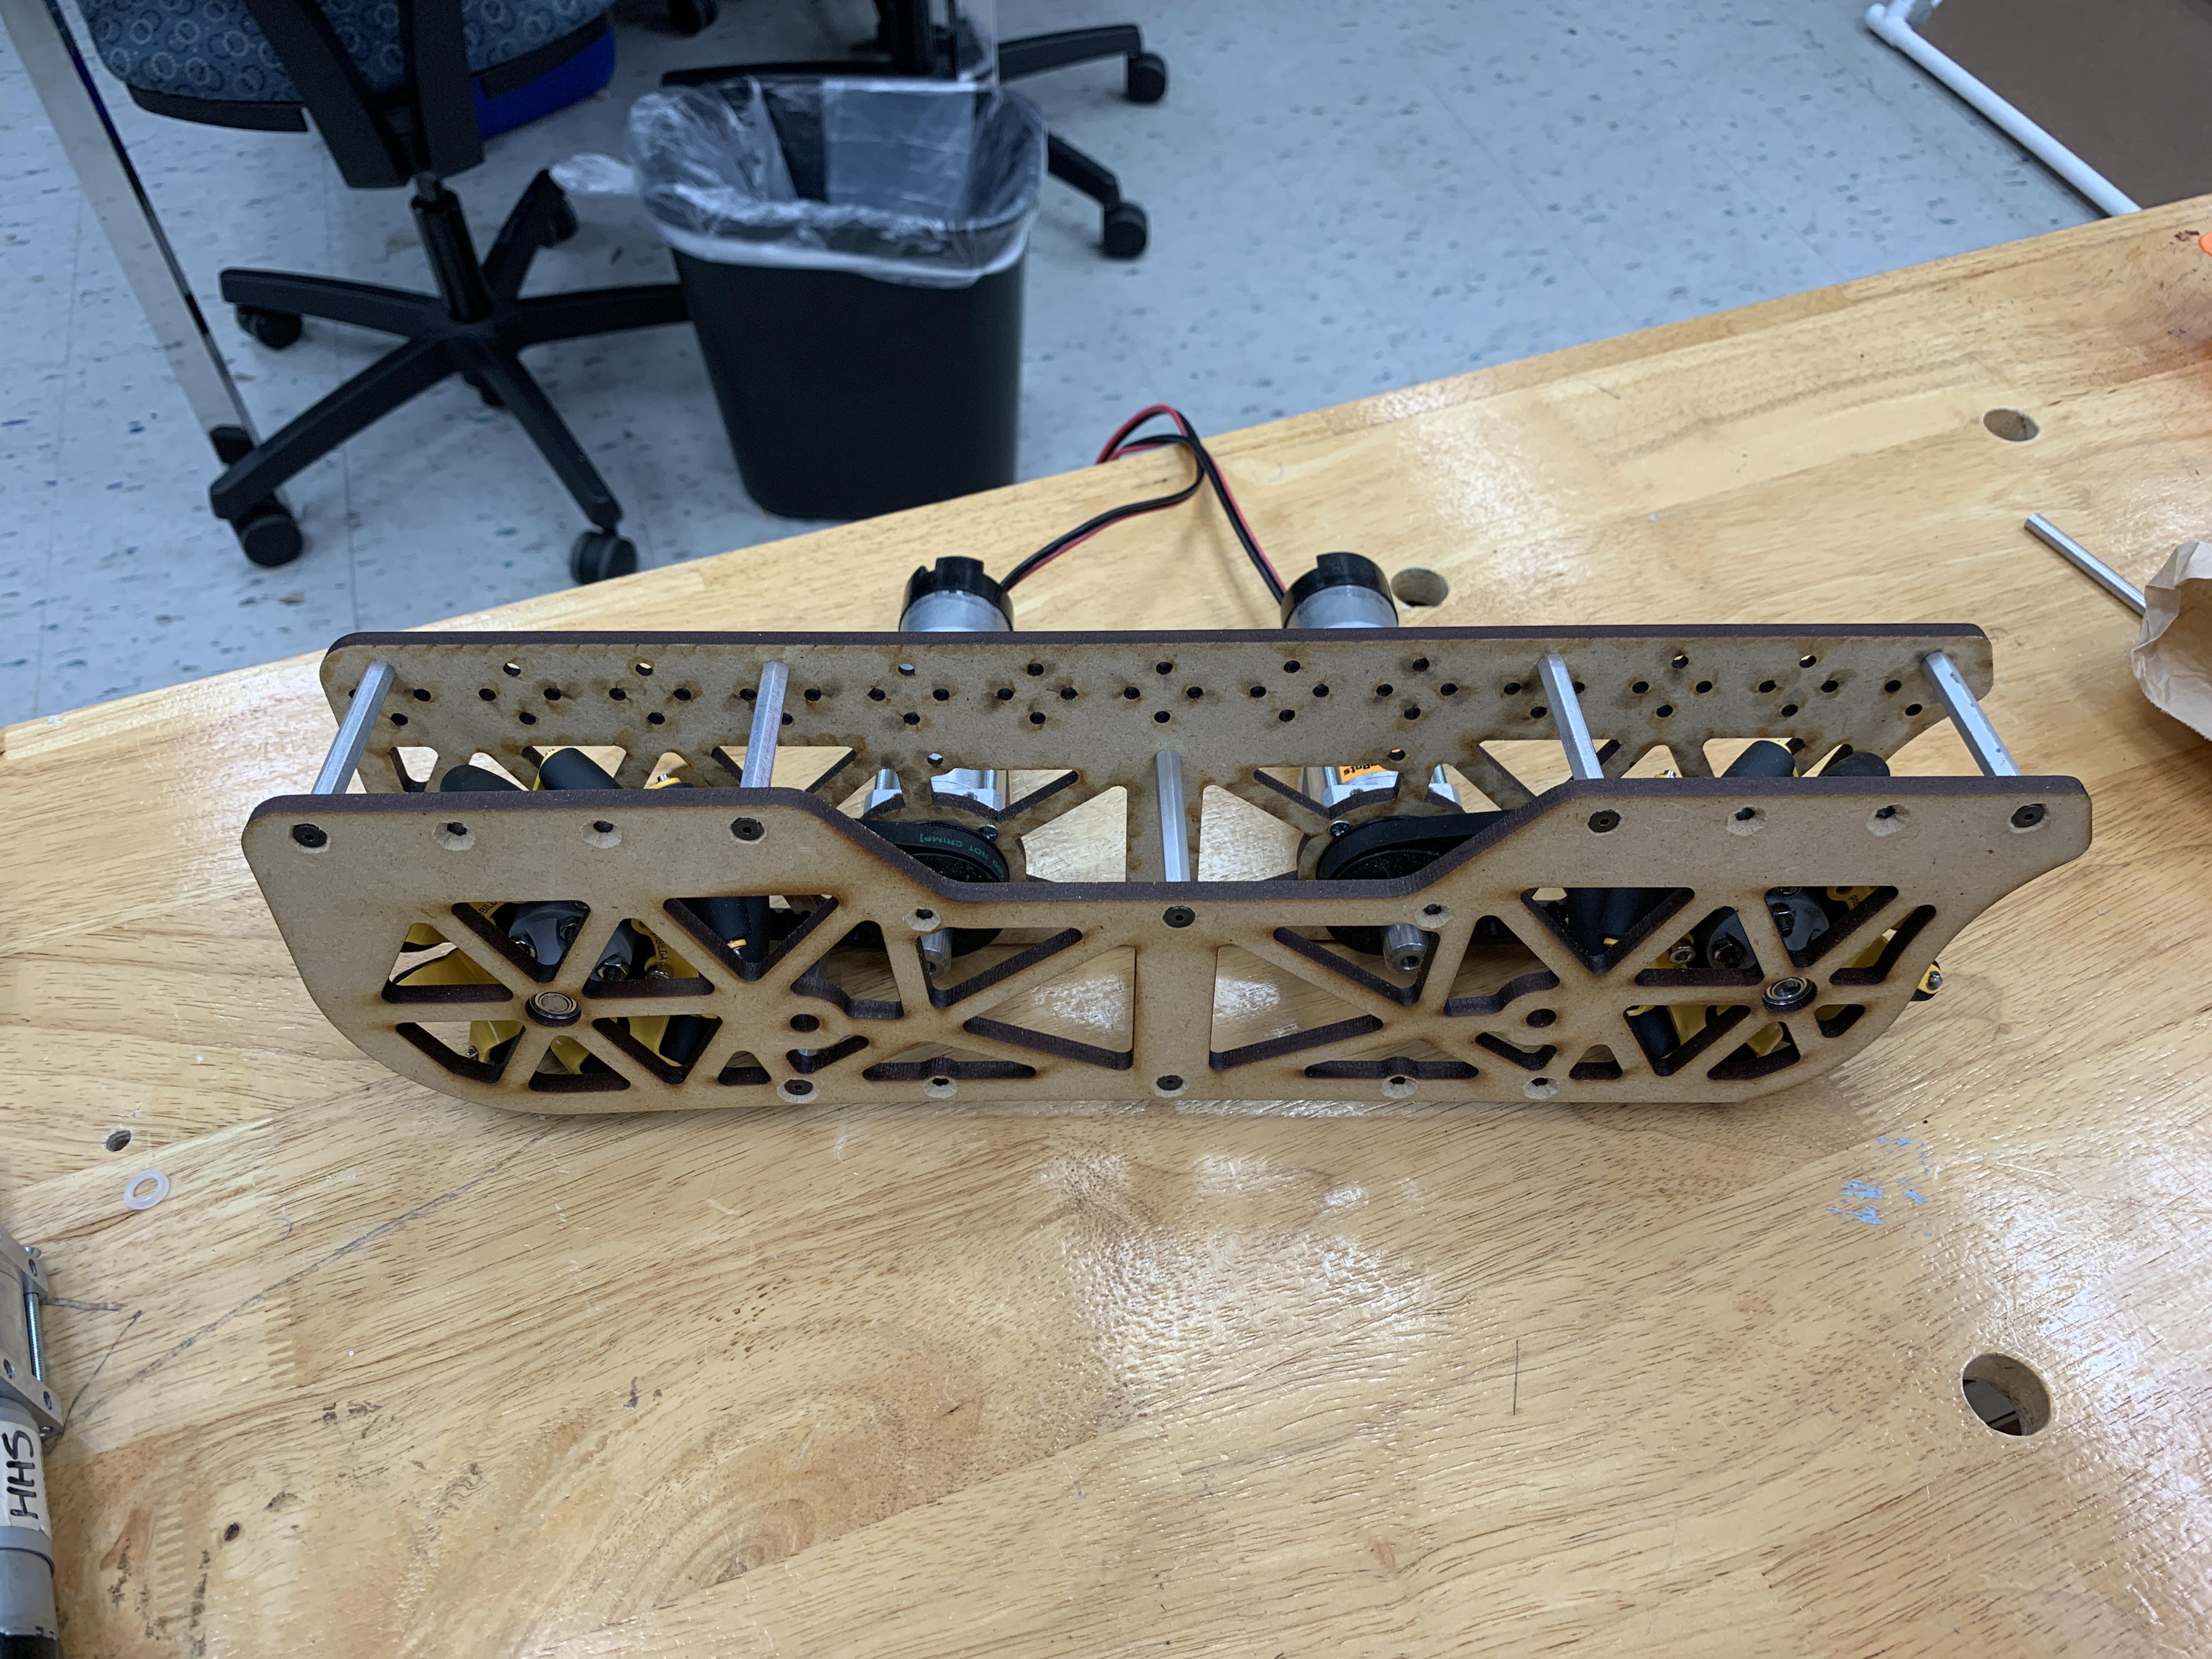
\includegraphics[width=0.9\textwidth, angle=0]{Meetings/July/07-21-21/drivetrain_7-20-21-NathanForrer.jpg}
% \caption{First half of the drivetrain.}
% \label{fig:072121_1}
% \end{figure}

\whatsnext{
\begin{itemize}
    \item Talk about the drivetrain
    
\end{itemize} 
}
